\documentclass[a4,notitlepage,12pt,spanish]{jedm}
%\usepackage[sc,sf,small]{titlesec}
\usepackage[table]{xcolor}
\usepackage{url}
\usepackage{graphicx}
% \usepackage{acmtrans}

\renewcommand{\figurename}{Figura}

\begin{document}

\title{Breve an\'alisis}
\date{}

\author{{\large Alejandro Lopez}\\alopezgjo@outlook.dom }

\maketitle


\section{Comparativa respecto a total} \label{sec:comparativa}

Es posible analizar la contribuci\'on de cada vertical al total de puntos redimidos usando una normalizaci\'on respecto a los puntos totales redimidos normalizados. En la Figura~\ref{fig:total} podemos seguir el comportamiento de cada vertical en el tiempo y sopesar su contribuci\'on al total de puntos redimidos; esto facilita identificar las temporadas que benefician o perjudican a cada vertical de manera visual.

\begin{figure}[!htb]
\centering
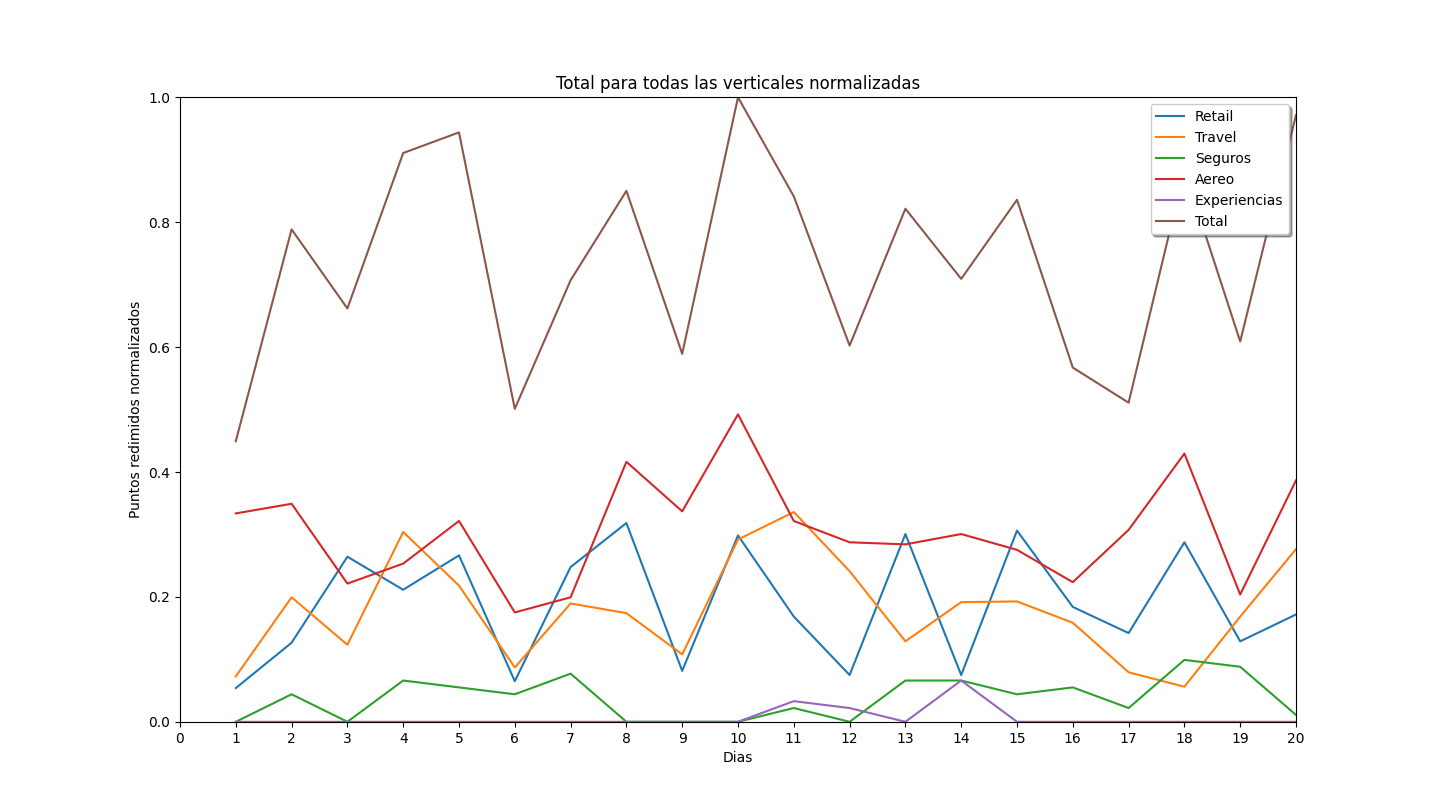
\includegraphics[scale=0.5]{total}
\caption{Comparativa entre puntos totales y verticales.}
\label{fig:total}
\end{figure}

De igual forma, se puede aplicar este procedimiento a una vertical en particular (ver Figura~\ref{fig:retail}).

\begin{figure}[!htb]
\centering
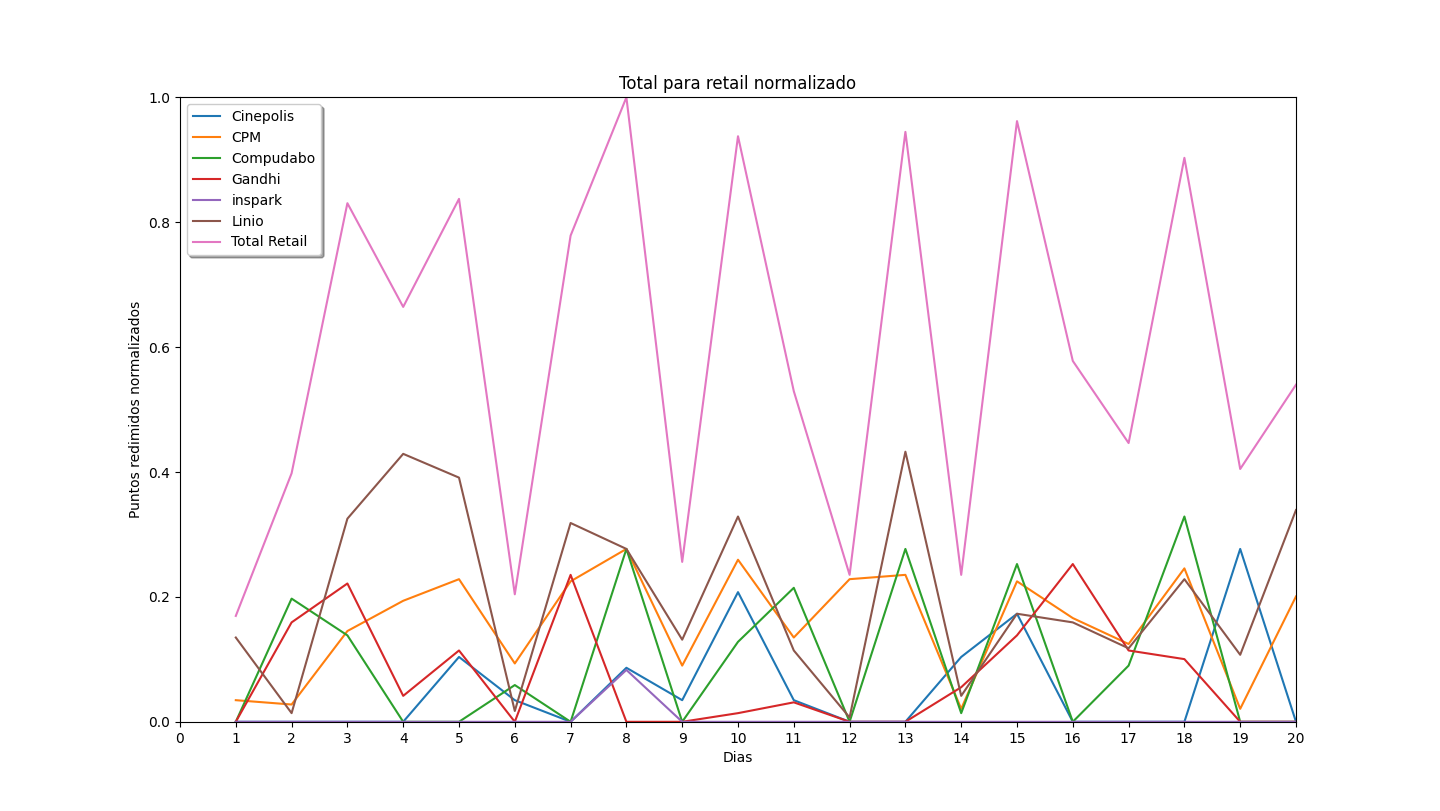
\includegraphics[scale=0.5]{retail}
\caption{Como en Figura~\ref{fig:total} pero para la vertical Retail.}
\label{fig:retail}
\end{figure}

\section{Predicci\'on con an\'alisis lineal} \label{sec:lineal}

La regresi\'on lineal es una herramienta muy \'util para predecir el comportamiento de una variable dependiente respecto a una variable independiente (caso simple). En la Figura~\ref{fig:regresion} se muestra un ajuste lineal de la dependencia de los puntos totales redimidos y los d\'ias. Se puede observar que no hay una fuerte dependencia dado que la pendiente de la recta (l\'inea azul continua) es cercana a cero; una de las razones por las que no existe una clara correlaci\'on es que la muestra de datos es bastante peque\~na (s\'olo 20 d\'ias), adem\'as de que la redenci\'on de puntos suele tener temporadas de auge y ocaso, por ejemplo, las vacaciones de verano son temporada de auge para los hoteles y agencias de viaje. 

\begin{figure}[!htb]
\centering
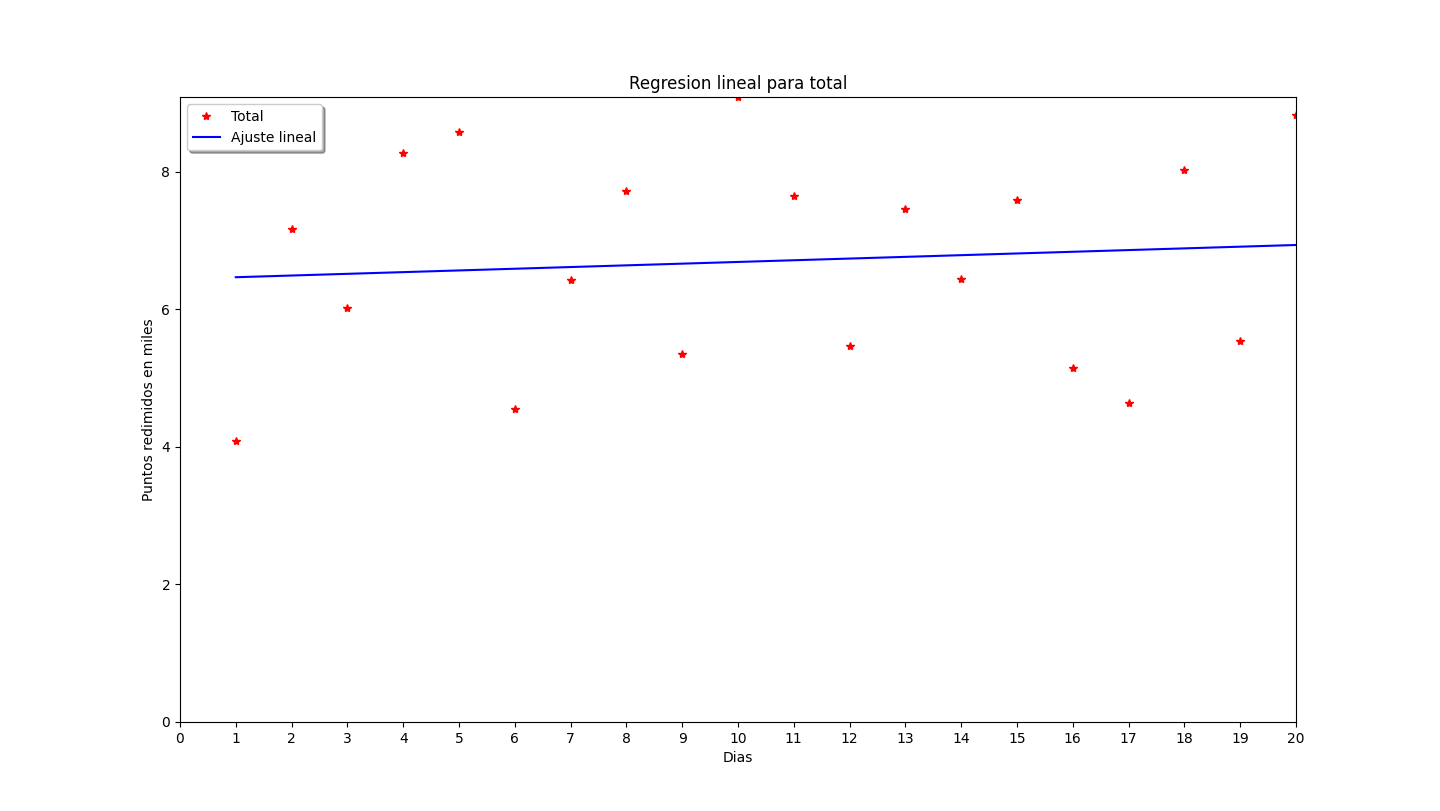
\includegraphics[scale=0.4]{regresion}
\caption{Regresi\'on lineal para la redenci\'on total de puntos en enero.}
\label{fig:regresion}
\end{figure}

Este tipo de an\'alisis lo podemos aplicar a cualquier vertical o registro de los datos. Por ejemplo, la Figura~\ref{fig:regresion_cine} muestra la predicci\'on para la cadena Cin\'epolis de la vertical Retail. Se observa que el ajuste tiene una correlaci\'on positiva para los d\'ias finales de enero. Esto puede indicar que la compra de boletos seguir\'a siendo marginalmente buena en los siguientes d\'ias. Sin embargo, hay que tener en cuenta que la compra de boletos para el cine est\'a relacionada con muchos otros factores: el d\'ia de la semana, fechas de estrenos esperados, d\'ias de asueto o especiales (14 de febrero), entre otros. Se puede mejorar este an\'alisis realizando un regresi\'on multilineal, pero esta requiere de una gran muestra de datos, adem\'as de variedad en los datos.

\begin{figure}[!htb]
\centering
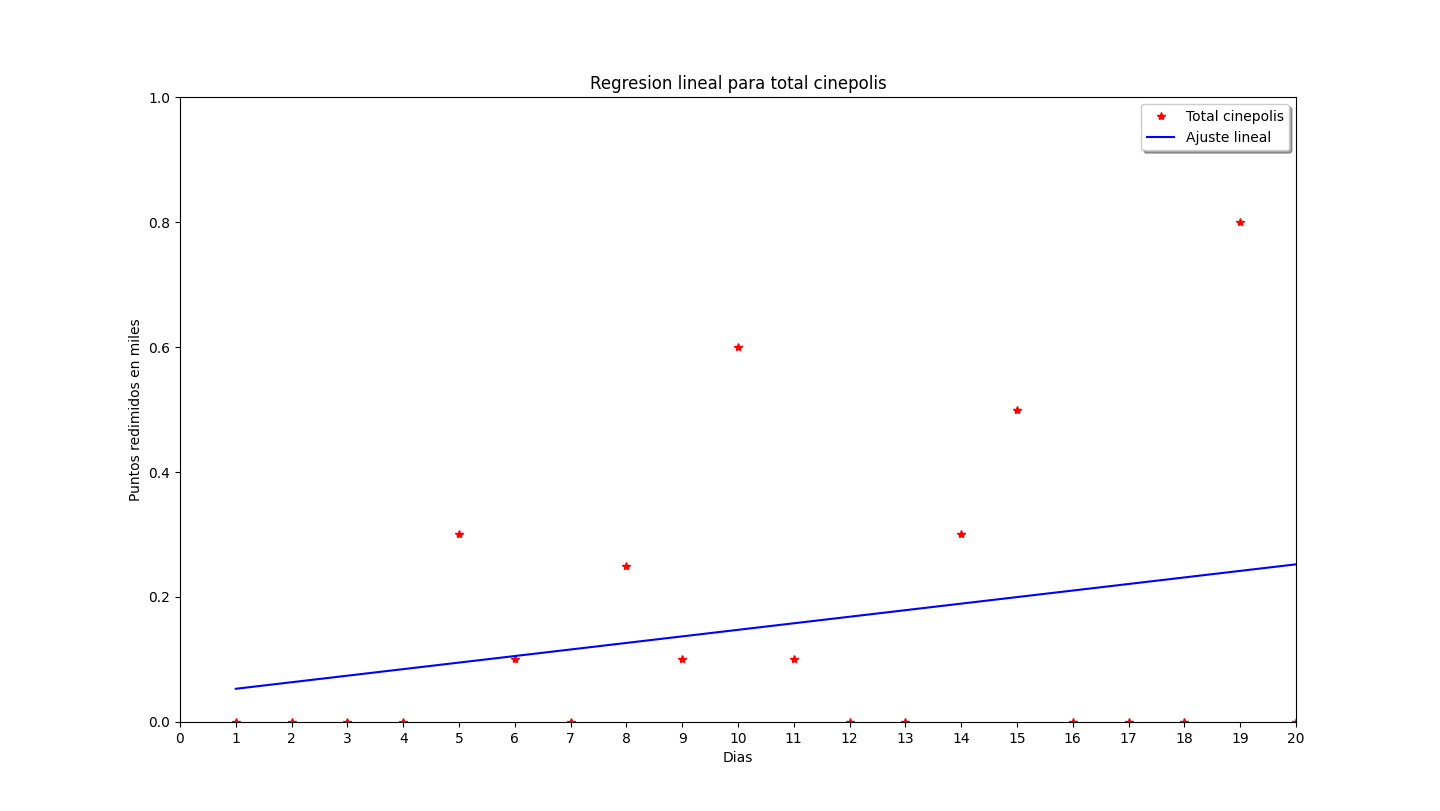
\includegraphics[scale=0.4]{regresion_cine}
\caption{Regresi\'on lineal para la redenci\'on de Cin\'epolis.}
\label{fig:regresion_cine}
\end{figure} 

\end{document}
